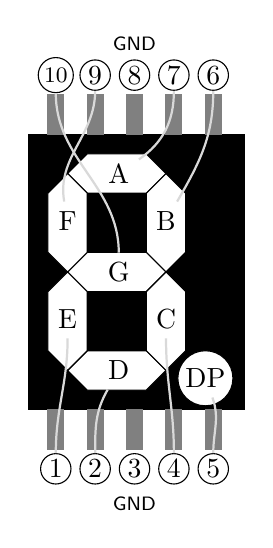
\begin{tikzpicture}[scale=0.5]
	% Rahmen der Anzeige
	\draw [fill=black] (0,0) rectangle (5.5,7);
	% Segment D
	\draw [fill = white] (1,1) -- ++(0.5,-0.5) -- ++ (1.5,0) -- ++ (0.5,0.5) -- ++ (-0.5,0.5) -- ++ (-1.5,0) -- ++(-0.5,-0.5)  node at ++(1.3,0) (segD) {D}; 
	% Segment G
	\draw [fill = white] (1,3.5) -- ++(0.5,-0.5) -- ++ (1.5,0) -- ++ (0.5,0.5) -- ++ (-0.5,0.5) -- ++ (-1.5,0) -- ++(-0.5,-0.5)  node at ++(1.3,0) (segG) {G};
	% Segment A
	\draw [fill = white] (1,6) -- ++(0.5,-0.5) -- ++ (1.5,0) -- ++ (0.5,0.5) -- ++ (-0.5,0.5) -- ++ (-1.5,0) -- ++(-0.5,-0.5)  node at ++(1.3,0) (segA) {A};
	% Segment E
	\draw [fill = white] (1,1) -- ++ (0.5,0.5) -- ++ (0,1.5) -- ++ (-0.5,0.5) -- ++ (-0.5,-0.5) -- ++ (0,-1.5) -- ++ (0.5,-0.5) node at ++ (0,1.3) (segE) {E};  
	% Segment C
	\draw [fill = white] (3.5,1) -- ++ (0.5,0.5) -- ++ (0,1.5) -- ++ (-0.5,0.5) -- ++ (-0.5,-0.5) -- ++ (0,-1.5) -- ++ (0.5,-0.5) node at ++ (0,1.3) (segC) {C};
	% Segment F
	\draw [fill = white] (1,3.5) -- ++ (0.5,0.5) -- ++ (0,1.5) -- ++ (-0.5,0.5) -- ++ (-0.5,-0.5) -- ++ (0,-1.5) -- ++ (0.5,-0.5) node at ++ (0,1.3) (segF) {F};
	% Segment B
	\draw [fill = white] (3.5,3.5) -- ++ (0.5,0.5) -- ++ (0,1.5) -- ++ (-0.5,0.5) -- ++ (-0.5,-0.5) -- ++ (0,-1.5) -- ++ (0.5,-0.5) node at ++ (0,1.3) (segB) {B};
	% Punkt DP
	\draw [fill = white] (4.5,0.8) circle [radius=0.7cm] node (segDP) {DP};
	% Kontaktstifte
	\foreach \x in {0.5, 1.5, ..., 4.5} {
		\draw [draw=gray, fill=gray] (\x,0) rectangle ++(0.4,-1);
		\draw [draw=gray, fill=gray] (\x,7) rectangle ++(0.4,1);
	}
	% Nummerierung der Kontaktstifte
	\node at (1-0.3,-1.5) [circle, draw, inner sep=1pt] (pin1) {1};
	\node at (2-0.3,-1.5) [circle, draw, inner sep=1pt] (pin2) {2};
	\node at (3-0.3,-1.5) [circle, draw, inner sep=1pt] (pin3) {3};
	\node at (4-0.3,-1.5) [circle, draw, inner sep=1pt] (pin4) {4};
	\node at (5-0.3,-1.5) [circle, draw, inner sep=1pt] (pin5) {5};
	%	\foreach \x in {9,...,6}{
	%		\node at (11-\x-0.3,8.5) [circle, draw, inner sep=1pt] {\x};
	%	}
	\node at (1-0.3,8.5) [circle, draw, inner sep=1pt] (pin10) {\footnotesize 10};
	\node at (11-9-0.3,8.5) [circle, draw, inner sep=1pt] (pin9) {9};
	\node at (11-8-0.3,8.5) [circle, draw, inner sep=1pt] (pin8) {8};
	\node at (11-7-0.3,8.5) [circle, draw, inner sep=1pt] (pin7) {7};
	\node at (11-6-0.3,8.5) [circle, draw, inner sep=1pt] (pin6) {6};
	\node at (2.7,-2.4) {\scriptsize\sffamily GND};
	\node at (2.7,9.3) {\scriptsize\sffamily GND};
	% Verbindungen
	\draw [gray!30!white, thick] (segA) to [out=35,in=270] (pin7); %out= Winkel beim Verlassen, in = Winkel beim Eintreffen
	\draw [gray!30!white, thick] (segB) to [out=60,in=270] (pin6);
	\draw [gray!30!white, thick] (segC) to [out=-90,in=90] (pin4);
	\draw [gray!30!white, thick] (segD) to [out=-120,in=90] (pin2);
	\draw [gray!30!white, thick] (segE) to [out=-90,in=90] (pin1);
	\draw [gray!30!white, thick] (segF) to [out=100,in=270] (pin9);
	\draw [gray!30!white, thick] (segG) to [out=90,in=270] (pin10);
	\draw [gray!30!white, thick] (segDP) to [out=-70,in=90] (pin5);
\end{tikzpicture}